\section{Nature of Delays}
\label{sec:nature_delays}

Many sub-cases can be studied from the general definition of a \gls{dmdp}. 
This section aims to give a bestiary of delays encountered in the literature or in practical \gls{rl} applications. We first present the different properties that can define a delay.
This section will be concluded with a presentation of the assumptions about the delay that will be made throughout this dissertation.

\begin{figure}[t]
    \centering
    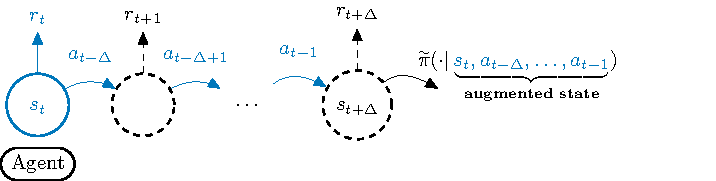
\includegraphics[bylabel=undelayedmdp]{img/thesis_plots.pdf}
    \caption{Representation of an undelayed \gls{mdp}.}
    \label{fig:undelayed_mdp}
\end{figure}

\subsection{Constant and Stochastic Delays}
\label{subsec:constant_stoch_delays}
As explained in the introduction, the delay is a random variable, but it is common to assume constant delays in the literature. 
This simplified model can be realistic enough for many applications, particularly if the potential stochasticity of the delay is negligible compared to the process' step size.
For example, \cite{ramstedt2019real} consider a 1-step constant delay for autonomous driving simulation and continuous robotic locomotion control; \cite{hester2013texplore} consider a 2-step delay for driving an autonomous vehicle; \cite{walsh2009learning} consider various delays between 1 and 20 on simple simulated tasks, including a grid world.
The delay can even go up to 63 steps for active flow control \cite{mao2022active}.
However, for some applications, the stochasticity of the delay must be modelled. 
In \cite{bouteiller2020reinforcement}, a stochastic delay is caused by the transmission of the policy via WiFi to a flying robot and the sending of the observation back.
\cite{campbell2016multiple} study the effect on Q-learning of Poisson distributed delay. 
In general, even though the real delay is not generally constant, the assumption of constant delay is made to simplify the problem, provided its variations in delay are not critical to the model's performance.

\subsection{State Observation and Action Execution Delays}
\label{subsec:state_action_delays}
\emph{State observation delay} manifest itself when the agent is no longer aware of the current state but has access to the past states of the \gls{mdp}. 
This contrasts with \gls{pomdp}, where past states are usually never disclosed to the agent, but instead, some partial information about the current state is revealed. \Cref{fig:state_obs_delayed_mdp} shows an example of state observation delay as opposed to an undelayed \gls{mdp} represented in \Cref{fig:undelayed_mdp}. 
In the figure, the reader may also notice the mention of \emph{augmented state}, which is the concatenation of the last observed state, $s_{t-\delay}$, and all the actions that the agent has selected in the past but whose outcome the agent has not to observed yet, $a_{t-\delay},\dots,a_{t-1}$. 
This notion is central to delayed reinforcement learning. 
Indeed, by considering the augmented state, the agent gathers all the possible information about the delayed process. 
Considering older states or actions than $s_{t-\delay}$ and $a_{t-\delay}$ would be redundant under the Markovianity property.

\emph{Action execution delay} occurs when the agent, albeit observing the current state, selects an action that will be executed only a few steps away from now in the future.
\Cref{fig:action_exec_delayed_mdp} shows an example of an action execution delay.
Note also the definition of the augmented state in this case.
Similarly to state observation delays, the augmented state exhaustively describes the delayed environment.
Another interesting point is about the time index. 
For action execution delay, the agent chooses at time $t$ an action labelled $a_t$. 
Due to the delay, this action will be applied at time $t+\delay$, to state $s_{t+\delay}$.
This is in contrast to the state observation delay, where the agent selects an action $a_t$ at time $t$ that will apply to the currently unobserved state $s_t$.
For constant delay, one could shift the action index by $\delay$ to ensure that action $a_t$ applies to $s_t$ as in an undelayed \gls{mdp}. 
However, this is only possible for constantly delayed \gls{mdp}. 
If the delay happened to be stochastic, then, the label of the action selected by the agent at time $t$ would be stochastic.
Moreover, if two actions applied at the same time due to the random delay, they would be given the same index. 
This doesn't seem to be a great nomenclature.
Therefore, in any case, we use the time when the agent selected an action for the index of this action.
Another advantage of this notation is the fact that the augmented state is the same in the case of state observation delay and action execution delay as evidentiated by \Cref{fig:state_obs_delayed_mdp} and \Cref{fig:action_exec_delayed_mdp}.

\begin{figure}[t]
    \centering
    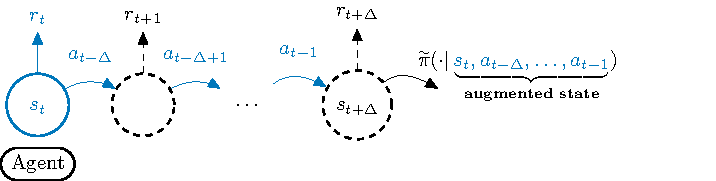
\includegraphics[bylabel=stateobsdelayedmdp]{img/thesis_plots.pdf}
    \caption{Representation of a \gls{dmdp} with state observation delay.}
    \label{fig:state_obs_delayed_mdp}
\end{figure}

\begin{figure}[t]
    \centering
    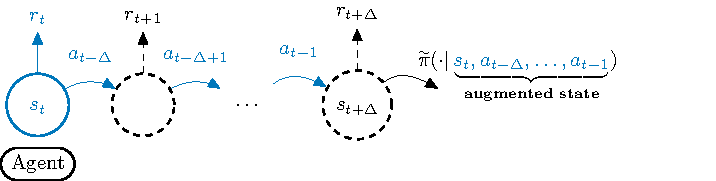
\includegraphics[bylabel=actionexecdelayedmdp]{img/thesis_plots.pdf}
    \caption{Representation of a \gls{dmdp} with action execution delay.}
    \label{fig:action_exec_delayed_mdp}
\end{figure}

As we shall see later, the action execution and the state observation delays are equivalent, and their effect adds up (\Cref{subsubsec:equiv_action_state_delays}).
That is why we have intentionally represented the two types of delay in an analogous way in the figures presented above.
Their augmented state follows a similar construction and contains the same number of terms for the same amount of delay.
However, as we shall discuss now, there are some minor differences that do not impact theoretical analysis if confusion is avoided.
As noted by \cite{chen2021delay}, a little complication could arise regarding the action execution delay; the delay can be divided into two parts: action selection and action actuation. 
The first amounts to the time it takes for the agent to compute its action after observing the last state.
The second is the time it takes for the agent to effectively apply this action in the environment. 
The latter source of delay is what is traditionally called action execution delay, whereas the former source of delay could be problematic in practice.
Indeed, if the environment provides a new state to the agent while it is still computing its previous action--which occurs when the action selection delay is longer than the step of the environment--then the agent does not yet know its previous action.
This is a problem for augmented approaches that we have introduced previously and which we will discuss in more detail in \Cref{sec:related_works}.
These approaches base their action selection scheme on the previous actions.
Therefore, here, an action is missing from the set of previous actions.
The agent could wait before computing the next action, but then the delay will accumulate, and the number of missing actions will increase.
To avoid such a scenario, we assume that the action selection delay is smaller than the step of the \gls{mdp} in this dissertation\footnote{If this is not the case in practice, then the action could be persisted for more steps to artificially create an \gls{mdp} with a longer step duration as in \cite{metelli2020control}.} as done in \cite{chen2021delay}.
Another difference between state and action delays is the effect of reward collection delays on state or action delays. 
As noted by \cite{katsikopoulos2003markov}, in the case of state observation delays, having no reward delay implies that the agent observes the outcome of a random variable correlated with the unobserved current state.
In fact, the current reward is a function of the unobserved current state.
Said alternatively, this setting provides partial information on the current unobserved state. 
Conversely, in the case of action execution delay, having no reward delay does not provide information to the agent since the most up-to-date information, the current state, is already known. 


\subsection{Reward Collection Delays}
\label{subsec:reward_delay}
A disambiguation might be needed. 
In the \gls{rl} literature, two different, although related, problems might be referred to as having delayed reward. 
In many real-life problems, it can be difficult to define a per-step reward, and instead, it can be easier to concentrate all the rewards in a single step \cite{han2022off}. 
For instance, it is hard to design a reward for each move in a chess match, while a reward of 0 or 1, depending on the result of the game, is much simpler.
This is the first type of delayed reward and can also be called \emph{sparse reward}. 
It usually involves a problem of exploration of the \gls{mdp}.
Instead, the second type of reward delay, which we call \emph{reward collection delays} appears when the reward associated with a transition--here, there is no problem in defining the per-step reward--is collected only after some steps have passed. 
As we will see, this type of delay is usually not relevant to \gls{rl} algorithms' final performance. 
Instead, it has an impact on learning speed.
The main difference between these two settings, therefore, lies in how the reward is designed in the first place. 
However, the first setting can be seen as an instance of the second, where all rewards are delayed and collected simultaneously in the final step. 


\subsection{Anonymous and Non-Anonymous Delays}
\label{subsec:anonymous_delays}
A distinction can be made between \emph{anonymous} and \emph{non-anonymous} delays. 
When the delay is anonymous, the agent does not have access to the amount of the delay; the timestamp associated with the observed state may not be disclosed to the agent.
Therefore, the latter is no longer aware of which state is the most recent from all the states it observes; the action that has effectively been executed at the current time is unknown; the transition which generated the collected reward is not accessible. 
Therefore, anonymity raises credit assignment problems.
As we will see later (see \Cref{sec:related_works}) and to the best of our knowledge, there are no works in the literature that consider anonymity for state observation or action execution delays in \gls{rl}. 
Anonymous delays are considered in the case of reward collection delays, however.


\subsection{Non-Integer Delays}
\label{subsec:non_int_delays}
In this subsection, we describe how the delay could amount to a non-integer number of steps of the environment.
For simplicity, we assume constant delays.
For clarity of the exposition, we assume $\delay\in(0,1)$ but the general case of $\delay\in\realnumbers[\ge0]$ is a simple extension of this framework.
We consider an action execution delay, but, as we will later see, the state observation delay is equivalent and can be similarly defined. 

To build a process with non-integer delay, one can start from a continuous-time stationary \gls{mdp}. 
As in \cite{sutton1999between}, if the agent can only observe the environment every unit of time, that is, at times $0,1,\dots,t,t+1,\dots$, then the discrete process that arises is a discrete-time \gls{mdp}. 
We call it $\markovdecisionprocess$. 
If, instead, the agent observes at the same frequency but with a phase shift of $\delay$, the time indices become $\delay,1+\delay,\dots,t+\delay,t+1+\delay,\dots$. 
Similarly, this defines a discrete time \gls{mdp} that we call $\markovdecisionprocess_\delay$. 
By the stationarity of the underlying continuous-time \gls{mdp}, $\markovdecisionprocess$ and $\markovdecisionprocess_\delay$ have the same transition and reward distribution. 
We now show how to build a $\delay$-delayed process using these two interleaved \glspl{mdp}.

Due to the action execution delay, the agent observes a state $s_t$ from $\mathcal{M}$ but its action $a_t$ will apply to a state $s_{t+\delay}$ of $\mathcal{M}_\delay$ that yields a reward of $r(s_{t+\delay},a_t)$. 
Transition probabilities are, of course, also affected. 
Anticipating the notation of \Cref{subsubsec:theory_augmented_space}, we define $\augmentedbelief(s_{t+\delay}\vert s_t,a)$ to be the probability of the transition from $s_t$ to $s_{t+\delay}$ after applying the action $a$ for $\delay$ units of time in the continuous time \gls{mdp}.

Because the continuous time underlying \gls{mdp} is stationary, one has $\forall(s,a,s')\in\statespace\times\actionspace\times\statespace$,
\begin{align}
    p(s'\vert s,a)=\int_{\statespace}   \augmentedbelief[1-\delay](s'\vert z,a)\augmentedbelief(z|s,a)\de z.\label{eq:def_p_non_int}
\end{align}
A visual representation of non-integer delays is given in \Cref{fig:non_int_delay_def}.


\begin{figure}[t]
    \centering
    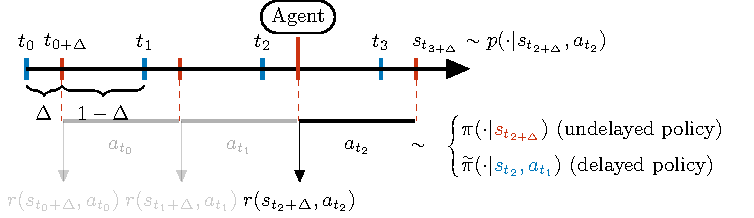
\includegraphics[labelimitation=nonintdelayedmdp]{img/thesis_plots_imitation.pdf}
    \caption{Representation of a \gls{dmdp} with non-integer action execution delay.}
    \label{fig:non_int_delay_def}
\end{figure}





%=============================================
% State-Dependent Delays
%---------------------------------------------
\subsection{State-Dependent and Action-Dependent Delays}
In this setting, the delay is no longer independent of the agent's behaviour. 
Either directly through the action or indirectly through the state, the agent might change the value of the delay.
To the best of our knowledge, no works in the \gls{rl} literature deal with state-dependent or action-dependent delays, yet practical applications inspire this problem. 
For example, using more complex policies to select actions might provide a better return if the computational time of such policies is reasonable. When this computational time grows too large, using a lighter policy to select actions may be reasonable. 
As another example, taking the setting of WiFi transmission to a flying robot of \cite{bouteiller2020reinforcement}, the delay could well depend on the distance from the robot to the policy computer. 


\subsection{On the Initialisation of Delayed Process}
\label{subsec:delay_init}
The reader may wonder how a delayed process is initialised.
For instance, in a state observation delay, how is the first set of states defined so that the agent effectively observes a delayed state from the beginning? 

This problem may seem superficial, but it can have important practical effects, as we will see later. 
If only the collection of the reward is delayed, then keeping the initialisation of the underlying \gls{mdp} does not pose a problem. 
Instead, for action execution and state observation delays, initialisation implies that the initial $\delay$ actions have to be sampled in some way before the agent is allowed to select any action. 
An arbitrary but reasonable sampling scheme for discrete or bounded action sets is to sample uniformly from this set. 
This is the approach we have followed in all the experiments of this dissertation. 

Note that depending on how the initial actions are sampled and whether the rewards collected in this initial phase are counted or not, the final return of the agent may change substantially.
As an illustration, consider the following simple example of an \gls{mdp} where the reward is equal to the speed of the agent and where there is only one action: ``accelerating'' of a fixed quantity. 
In the \gls{dmdp}, the initialisation implies that the action ``accelerating'' is applied several times before the control is left to the agent.
This means that in its current unobserved state, the agent has already accumulated speed compared to the undelayed agent, whose initialisation sets him at speed 0.
Even if the rewards in the initialisation are not counted, the delayed agent starts with more speed and therefore collects higher rewards than the undelayed one.
Besides, if the rewards are counted during the initialisation, then the delayed agent accumulates even more reward.
Therefore, the way the rewards are counted can drastically change the return of the delayed agent with respect to the undelayed one.
We call this effect the \emph{delay initialisation shift}.



